\chapter{Differential forms}\label{ch:differential-forms}
\begin{chout}
	The following chapter gives an exposition of the basics of differential forms
	on manifolds, following Bott--Tu\sidenotemark. In this way, it is written with
	the same motivation as Chapter~\ref{ch:manifold-theory}; we will conclude with
	specification to Riemann surfaces.
\end{chout}
\sidenotetext[][5\baselineskip]{\footnotesize\cite{bott}}

\section{Differential forms on $ \mathbb{R}^{2} $}
Before considering what it means to integrate a function on a Riemann surface,
or even a smooth manifold, we develop the theory of differential forms in the
real plane. Differential forms provide an alternative framework to that of
vector calculus; one which is often considered to be more simple and
flexible\sidenote{\footnotesize\cite{tu}}. Let $ x_1, x_2 $ be the standard
coordinates on $ \mathbb{R}^{2} $ and denote by $ \Omega ^{*} $ the space
generated by $ \d{x_1}, \d{x_2} $, governed by the relations,
\begin{gather*}
	\d{x_i}\d{x_i} = 0,\\
	\d{x_1}\d{x_2} = - \d{x_2}\d{x_1}.
\end{gather*}

\begin{remark}
	The space $ \Omega ^{*} $ can be regarded as a vector space over $ \mathbb{R}
	$, and has the basis,
	\begin{align*}
		1, \d{x_1}, \d{x_2}, \d{x_1}\d{x_2}.
	\end{align*}
\end{remark}

\begin{definition}[Differential forms\sidenotemark]
	With $ \Omega ^{*} $ as above, the \defined{$ C ^{\infty} $ differential forms}
	are elements of,
	\begin{align*}
		\Omega ^{*}\left(\mathbb{R}^{2}\right) = \left\{ C ^{\infty} \text{
			functions on } \mathbb{R}^{2} \right\} \otimes _{\mathbb{R}} \Omega ^{*}
	\end{align*}
	where $ \otimes _{\mathbb{R}} $ denotes the tensor product over $ \mathbb{R}
	$.
\end{definition}
\sidenotetext[][-7\baselineskip]{\footnotesize\cite[p.13]{bott}}

\begin{remark}
	A differential form is simply an expression of the form,
	\begin{align*}
		\omega = \sum_{I}^{}{f _{I} \d{x_I}}
	\end{align*}
	where $ I $ denotes a multi-index, and the $ f_I $ are smooth.
\end{remark}

There is also a natural decomposition (or
grading\sidenote{\footnotesize\cite[p. 13]{bott}}) of the space $ \Omega
	^{*}(\mathbb{R}^{2}) $ as,
\begin{align*}
	\Omega ^{*}( \mathbb{R}^{2}) = \bigoplus_{i=0}^{2}{\Omega
	^{i}(\mathbb{R}^{2})}
\end{align*}
where the space $ \Omega^i(\mathbb{R}^{2}) $ contains the $ i $-forms, over $
	\mathbb{R}^{2} $. To dispense with abstraction, the space $
	\Omega^1(\mathbb{R}^{2}) $ can be recognised as,
\begin{align*}
	\Omega^1(\mathbb{R}^{2}) = \left\{ f(x,y)\d{x} + g(x,y)\d{y}:
	f,g \in C ^{\infty}\left( \mathbb{R}^{2} \right) \right\}.
\end{align*}

Furthermore, we can naturally define a differential operator $ \d{} $ which acts
between these subspaces.

\begin{definition}[Exterior derivative]
	We define the \defined{exterior derivative} to be the differential operator,
	\begin{align*}
		\d : \Omega^i(\mathbb{R}^{2}) \to \Omega ^{i+1}(\mathbb{R}^{2})
	\end{align*}
	with the following conditions.
	\begin{enumerate}
		\item If $ f \in \Omega^0(\mathbb{R}^{2}) $, then,
		      \begin{align*}
			      \d{f} = \frac{\partial f}{\partial x}\d{x} + \frac{\partial f}{\partial
				      y}\d{y}.
		      \end{align*}
		\item If $ \omega \in \Omega ^{*}(\mathbb{R}^{2}) $ can be expressed as $
			      \omega = \sum_{}^{}{f _{I} \d{x_I}} $ for multi-index $ I $,
		      \begin{align*}
			      \d{\omega} = \sum_{}^{}{\d{f_I}\d{x_I}}.
		      \end{align*}
	\end{enumerate}
\end{definition}

\begin{proposition}
	$ \d{}^2=0 $.
	\begin{proof}
		Let us first consider concretely the form of the operator $ \d $ in our
		context. We are given the form of the operator $ d: \Omega^0(\mathbb{R}^{2})
			\to \Omega^1(\mathbb{R}^{2}) $ in the definition, so it remains to consider
		the form of the operator as a function between $ \Omega^1(\mathbb{R}^{2}) $
		and $ \Omega^2(\mathbb{R}^{2}) $.

		Suppose that $ \omega \in \Omega^1(\mathbb{R}^{2}) $, expressible as $ f_1
			\d{x_1} + f_2 \d{x_2} $ for smooth $ 0 $-forms $ f_1,f_2 $. Then,
		\begin{align*}
			\d{\omega} & = \d \left( f_1 \d{x_1} + f_2 \d{x_2} \right)              \\
			           & = \left( \frac{\partial f_1}{\partial x_1}\d{x_1} +
			\frac{\partial f_1}{\partial x_2}\d{x_2} \right)\d{x_1} +
			\left( \frac{\partial f_2}{\partial x_1}\d{x_1} +
			\frac{\partial f_2}{\partial x_2}\d{x_2} \right)\d{x_2}                 \\
			           & = \frac{\partial f_1}{\partial x_2}\d{x_2}\d{x_1} +
			\frac{\partial f_2}{\partial x_1}\d{x_1}\d{x_2}                         \\
			           & = \left( \frac{\partial f_2}{\partial x_1}- \frac{\partial
				f_1}{\partial x_2} \right)\d{x_1}\d{x_2}
		\end{align*}
		using the fact that $ \d{x_1}\d{x_2}= -\d{x_2}\d{x_1} $.

		At this point, we also note that for $ \mathbb{R}^{2} $ the operator $
			\d{}^{2} $ can only act between $ \Omega^0 $ and $ \Omega^2 $. Hence, we
		consider a smooth function $ f $,
		\begin{align*}
			\d{} \circ \d{f} & = \d \left( \frac{\partial f}{\partial x_1}\d{x_1} +
			\frac{\partial f}{\partial x_2}\d{x_2} \right)                             \\
			                 & = \left( \frac{\partial f}{\partial x_1 \partial x_2} -
			\frac{\partial f}{\partial x_2 \partial x_1}\right) = 0
		\end{align*}
		with the final equality a consequence of the interchangeabiliy of partial
		derivatives for smooth functions (Clairaut's Theorem).
	\end{proof}
\end{proposition}

There is another important operation on differential forms, called the
wedge/exterior product, which is easily defined in our framework.

\begin{definition}[Exterior product]
	Let $ \sigma, \tau \in \Omega ^{*}(\mathbb{R}^{2}) $, be representable as $
		\sum_{I}^{}{f_I \d{x_I}} $ and $ \sum_{J}^{}{g_J \d{x_J}} $ for
	multi-indices $ I,J $ respectively. Then, we define the \defined{exterior
		product} of $ \sigma $ and $ \tau $, to be the operation,
	\begin{align*}
		\sigma \wedge \tau = \sum_{I}^{}{f_I \d{x_I}}\wedge \sum_{J}^{}{g_J
		\d{x_J}} = \sum_{I,J}^{}{f_I g_J \d{x_I}\d{x_J}}.
	\end{align*}
\end{definition}

\begin{example}
	We consider the case of $ \sigma, \tau \in \Omega^1(\mathbb{R}^{2}) $. Let $
		\sigma = f_1 \d{x_1}+f_2 \d{x_2} $ and $ \tau = g_1 \d{x_1}+g_2 \d{x_2} $.
	Then,
	\begin{align*}
		\sigma \wedge \tau & = \left( f_1 \d{x_1} + f_2 \d{x_2} \right)\wedge \left(
		g_1 \d{x_1}+ g_2 \d{x_2} \right)                                             \\
		                   & = f_1 g_1 \d{x_1}\d{x_1} + f_1 g_2 \d{x_1}\d{x_2} + f_2
		g_1 \d{x_2}\d{x_1} + f_2 g_2 \d{x_2}\d{x_2}                                  \\
		                   & = f_1 g_2 \d{x_1}\d{x_2} + f_2 g_1 \d{x_2}\d{x_1}       \\
		                   & = \left( f_1 g_2 - f_2 g_1 \right)\d{x_1}\d{x_2}
	\end{align*}
	with each simplification justified by the original defining relations of the
	$ \d{x_i} $.
\end{example}

\subsection{The de Rham complex}
In a somewhat implicit manner, we have introduced a cohomological concept, with
further reaching consequences, than the one we initial desired. The differential
operator $ \d{} $ together with $ \Omega ^{*} $, defines the \defined{de Rham
	complex} on $ \mathbb{R}^{2} $ (and by extension $ \mathbb{R}^{n} $). In a more
general treatment, the de Rham complex is an example of a \defined{differential
	complex} since it can be expressed as a direct sum of vector spaces $ \Omega
	^{*} = \bigoplus_{i=0}^{2}{\Omega^i} $ where there are sequential homomorphisms
defined by the operator $ \d{} $ such that $ \d{}^{2}=0 $.

\begin{marginfigure}
	\centering
	\includegraphics{de-rham/figure}
	\caption{The de Rham complex on $ \mathbb{R}^{2} $.}
\end{marginfigure}

\begin{definition}[de Rham cohomology groups]
	We define the $ i $th \defined{de Rham cohomology group} on $ \mathbb{R}^{n} $
	to be the vector space,
	\begin{align*}
		H^i \left( \mathbb{R}^{n} \right) = \frac{\ker \left( \d{}:
			\Omega^i\left(\mathbb{R}^{2}\right) \to \Omega
			^{i+1}\left(\mathbb{R}^{2}\right) \right)}{\im\left( \d{}: \Omega
			^{i-1}\left(\mathbb{R}^{2}\right) \to
			\Omega^i\left(\mathbb{R}^{2}\right) \right)}.
	\end{align*}
\end{definition}

Of course, we are mostly interested in $ \mathbb{R}^{2} $, and the definition
can be easily specified to this account. We refer to the differential forms
contained in the above kernel as \defined{exact}, and those contained in the
image as \defined{closed}.

\section{Differential forms on smooth manifolds}
Since manifolds are by definition locally Euclidean, we aim to transport our
ideas about differential forms in $ \mathbb{R}^{2} $ into the manifold setting
using the charts and coordinate functions which define the manifold structure.

\begin{definition}[Pullback]
	Let $ u_1, u_2 $ and $ v_1, v_2 $ be standard coordinate systems on two
	subsets $ U, V \subseteq \mathbb{R}^{2} $. For a $ C ^{\infty} $ function $
		f:U \to V $ we define the pullback map $ f ^{*} $ on $ 0 $-forms by,
	\begin{align*}
		f ^{*} & : \Omega^0(V) \to \Omega^0(U) \\
		       & : g \mapsto g \circ f.
	\end{align*}
\end{definition}

So for smooth maps, the pullback is nothing more than pre-composition by a
smooth function. We now aim to extend this idea to forms of higher order, that
is $ 1 $- and $ 2 $-forms. If we impose\sidenote{\footnotesize\cite[p.
		36]{bott}} that the differential operator $ \d{} $ should commute with the
operation of `pulling-back', there is a unique expression of $ f ^{*} $. Letting
$ U, V $ be as in the definition, consider a $ 1 $-form $ \omega \in \Omega^1(V)
$, expressible as $ \omega = \alpha \d{v_1} + \beta \d{v_2}$, for smooth
functions $ \alpha, \beta $. Then the pullback is defined as,
\begin{align*}
	f ^{*} & : \Omega^1(V) \to \Omega^1(U)                                        \\
	       & : \omega \mapsto \left( \alpha \circ f \right) \left( \frac{\partial
		v_1}{\partial u_1}\d{u_1} + \frac{\partial v_1}{\partial u_2}\d{u_2}
	\right)                                                                       \\
	       & \qquad\qquad + \left( \beta \circ f \right) \left( \frac{\partial
		v_2}{\partial u_1}\d{u_1} + \frac{\partial v_2}{\partial u_2}\d{u_2}
	\right).
\end{align*}

\begin{remark}
	Imposing that the operation of pulling-back should commute with the
	differential operator $ \d{} $ is equivalent to the assertion that $ \d{} $ is
	independent of the system of coordinates.
\end{remark}

\begin{definition}[Differential form]
	For a smooth manifold $ M $, defined by an atlas $ \{ U_i, \phi_i \} $, a
	\defined{$ C ^{\infty} $ differential form} is a collection of differential
	forms $ \{ \omega_i \} $, each defined on $ \tilde{U} _{i} $ such that
	\begin{align*}
		U_i \cap U_j \neq \varnothing \implies \phi_i ^{*} \omega_i = \phi_j
		^{*}\omega_j
	\end{align*}
	on the intersection.
\end{definition}

This is an intuitively logical extension of the theory, and while we won't
consider smooth manifolds anymore, $ C ^{\infty} $ forms will remain important,
even in the complex setting.

\section{Differential forms on Riemann surfaces}
Thus far, our development of differential forms has been independent of complex
structure. This complex structure is, however, integral to the definition of
Riemann surfaces and we can use it to further explore differential forms on
manifolds.

To begin with, we change our notation to one more in line with our complex
considerations. Consider a local coordinate $ z = x+iy $, and also the complex
conjugate $ \overline{z} = x - i y $. We can easily invert these relations,
\begin{align*}
	x = \frac{z + \overline{z}}{2},\qquad y = \frac{z - \overline{z}}{2i}
\end{align*}
and can equally well express any $ C ^{\infty} $ $ 1 $-form as,
\begin{align*}
	\omega = f(z, \overline{z}) \d{z} + g(z, \overline{z})\d{\overline{z}}.
\end{align*}

Further to this, we can define the partial differential operators in this
context by,
\begin{align*}
	\frac{\partial }{\partial z} = \frac{1}{2} \left( \frac{\partial }{\partial
		x}-i \frac{\partial }{\partial y} \right), \qquad
	\frac{\partial }{\partial \overline{z}} = \frac{1}{2}\left(
	\frac{\partial }{\partial x}+ i \frac{\partial }{\partial y} \right)
\end{align*}
which have associated differential operators,
\begin{align*}
	\partial = \frac{\partial }{\partial z}\d{z},\qquad
	\overline{\partial} = \frac{\partial }{\partial \overline{z}}\d{\overline{z}}.
\end{align*}

\begin{remark}
	The idea is that the additional complex structure can be summarised as a
	map $ \star: \Omega^1 \to \Omega^1 $ such that
	\begin{align*}
		\star \d{x} = \d{y}, \\
		\star \d{y} = - \d{x}.
	\end{align*}
	From this, we can see that $ \star^2=-1 $, and hence we can decompose the
	space of $ C ^{\infty} $ $ 1 $-forms into the eigenspaces of this operator.
\end{remark}

\begin{lemma}
	For the differential operators $ \d{}, \partial, \overline{\partial} $, we
	have the following identities,
	\begin{gather*}
		\d{} = \partial + \overline{\partial },\\
		\partial ^{2} = \overline{\partial }^{2} = \partial \overline{\partial }+
		\overline{\partial }\partial =0.
	\end{gather*}
\end{lemma}

\begin{notation}
	We denote by $ \Omega ^{1,0}(X) $ the space of differential $ 1 $-forms which
	are locally expressible as $ f(z,\overline{z})\d{z} $, and by $ \Omega
		^{0,1}(X) $ the space of differential forms locally expressible as $ g(z,
		\overline{z})\d{\overline{z}} $.

	This notation is particularly well chosen since it makes clear the fact that
	we are decomposing the space of smooth $ 1 $-forms $ \Omega^1(X) $.
\end{notation}

\begin{marginfigure}
	\centering
	\includegraphics{dolbeault/figure}
	\caption{Visualising the action of $ \partial $ and $ \overline{\partial} $.}
\end{marginfigure}

\begin{definition}[Holomorphic/Meromorphic form]
	A \defined{holomorphic $ 1 $-form} (\defined{meromorphic $ 1 $-form}) on a
	Riemann surface $ X $ is a form which can be locally expressed by,
	\begin{align*}
		\omega = f(z) \d{z}
	\end{align*}
	where $ f $ is holomorphic (meromorphic).
\end{definition}

\begin{definition}[Anti-holomorphic form]
	An \defined{anti-holomorphic $ 1 $-form} on a Riemann surface $ X $ is a form
	which can be locally expressed by,
	\begin{align*}
		\omega = g(z) \d{\overline{z}}
	\end{align*}
	where $ \overline{g(z)} $ is holomorphic.
\end{definition}

\begin{notation}
	It is common to denote the holomorphic $ 1 $-forms on a Riemann surface $ X $
	by $ \mathcal{O}^{1}(X) $, the meromorphic $ 1 $-forms by $
		\mathcal{M}^{1}(X) $, and the anti-holomorphic $ 1 $-forms by $
		\overline{\mathcal{O}^{1}}(X) $.
\end{notation}

There are two results, closely related, which we will need later.

\begin{proposition}\label{prop:hol}
	A smooth function $ f \in \Omega^0(X) $ is holomorphic if and only if $
		\overline{\partial }f=0 $.
	\begin{proof}
		Fixing a local coordinate $ z=x+iy $, we see that
		\begin{align*}
			\overline{\partial }f = 0 \iff
			\frac{\partial f}{\partial \overline{z}} \d{z}=0 \iff
			\frac{\partial f}{\partial x}+i \frac{\partial f}{\partial y}=0,
		\end{align*}
		which are exactly the Cauchy--Riemann equations for $ f $.
	\end{proof}
\end{proposition}

\begin{proposition}\label{prop:anti-hol}
	A smooth function $ g \in \Omega^0(X) $ is anti-holomorphic if and only if $
		\partial g=0 $.
\end{proposition}

These results, can be extended to the holomorphic and anti-holomorphic $ 1
$-forms, and in many cases\sidenote{\footnotesize\cite{forster}} the condition
that $ \overline{\partial }\alpha=0 $ is the defining condition for $ \alpha \in
	\mathcal{O}^{1}(X) $.

Recall that a key integer value associated to a meromorphic map was the order.
We can extend this notion to a meromorphic $ 1 $-forms as follows.

\begin{definition}[Order]
	Let $ p \in X $, $ \omega \in \mathcal{M}^{1}(X) $. Given a local coordinate
	$ z $ centred on $ p $, and a local representation of $ \omega $ as $ f ( z
		)\d{z} $, the \defined{order} of $ \omega $ is defined as,
	\begin{align*}
		\ord ( \omega;p ) = \ord ( f;0 ).
	\end{align*}
\end{definition}

There is a final result\sidenote{\footnotesize\cite[p.132]{miranda}} in the
realm of meromorphic forms and functions which will prove useful.

\begin{lemma}\label{lem:mero-1-forms}
	Let $ \omega_{1}, \omega_{2}\in \mathcal{M}^{1}( X ) $ with $ \omega_{1}
		\not\equiv 0 $. Then, there exists a unique function $ f \in \mathcal{M}( X )
	$ such that
	\begin{align*}
		\omega_{2} = f \omega_{1}.
	\end{align*}
	\begin{proof}
		Suppose that there exists a chart $ \phi:U \to \tilde{U} $ which gives a
		local coordinate $ z $, and suppose also that for $ i=1,2 $, $ \omega_{i} =
			g_{i}(z)\d{z} $, where $ g_{i} $ are meromorphic functions on $ \tilde{U} $.
		If we take $ f = ( g_{2}/g_{1} )\circ \phi $, this is a meromorphic function
		on $ U $, and has the desired property. Showing that this function is
		independent of coordinate chart is straightforward, and this is indeed the
		function we desired.
	\end{proof}
\end{lemma}

\subsection{The Dolbeault complex}
As for the de Rham complex with the differential operator $ \d{} $, we can
define the Dolbeault complex with the operator $ \overline{\partial} $, which
satisfies the conditions for a differential complex since $
	\overline{\partial}\circ\overline{\partial}=0 $. For our consideration, there
will be four particularly important vector spaces.

\begin{gather*}
	H ^{0,0}(X) = \ker \left( \overline{\partial}: \Omega^0 \to \Omega ^{0,1} \right)\\
	H ^{1,0}(X) = \ker \left( \overline{\partial}: \Omega ^{1,0} \to \Omega^2 \right)\\
	H ^{0,1}(X) = \coker \left( \overline{\partial}: \Omega^0 \to \Omega ^{0,1}
	\right) = \left. \Omega^{0}\middle/\im \left( \overline{\partial
	}:\Omega^{0}\to \Omega^{0,1} \right) \right.\\
	H ^{1,1}(X) = \coker \left( \overline{\partial}: \Omega ^{1,0} \to \Omega^2
	\right) = \left. \Omega^{1,0}\middle/\im \left( \overline{\partial }:
	\Omega^{1,0}\to \Omega^{2} \right) \right.
\end{gather*}

The importance of the last two of these spaces is not at all obvious, but the
first two can be easily understood as the spaces of holomorphic functions and
holomorphic $ 1 $-forms.

\section{Integration on Riemann surfaces}
The work of this chapter has all been motivated by the prospect of defining
integration on a Riemann surface, which is what we do now. As in complex
analysis, there are some fundamental results contained in this area. We have
defined the objects we want to integrate, i.e. $ 1 $- and $ 2 $-forms, so we now
define\sidenote{\footnotesize\cite[p. 118]{miranda}} the sets over which we want
to integrate.

\begin{definition}[Path]
	A \defined{path} on a Riemann surface $ X $ is a continuous, piecewise $ C
			^{\infty} $ function,
	\begin{align*}
		\gamma:[a,b]\subseteq \mathbb{R} \to X
	\end{align*}
	where the interval $ [a,b] $ is closed.
\end{definition}

\begin{remark}
	If $ \gamma(a)=\gamma(b) $, we call the path \defined{closed}. We call a path
	\defined{simple} if it is either closed and injective on $ [ a,b ) $, or
	injective.
\end{remark}

\begin{definition}[$ 1 $-form integration]
	Let $ X $ be a Riemann surface, $ \omega $ a $ C ^{\infty} $ $ 1 $-form on $ X
	$, and $ \gamma $ a path whose image is contained by the domain of a single
	chart in the atlas of $ X $, $ \phi:U \to \tilde{U} $. Suppose that $ \omega $
	can be locally represented by $ f \d{z} + g \d{\overline{z}} $ in $ U $. Then,
	the \defined{integral} of $ \omega $ along $ \gamma $ is,
	\begin{align*}
		\int_{\gamma}^{}{\omega} = \int_{\phi \gamma}^{}{f \d{z} + g
		\d{\overline{z}}}
	\end{align*}
	where the right-hand side integral is the standard contour integral.
\end{definition}

\begin{marginfigure}
	\centering
	\includegraphics{path/figure}
	\caption{The integral of $ 1 $-form over a path on a Riemann surface.}
\end{marginfigure}

It is fairly clear that any path on a $ X $ may be arbitrarily partitioned, and in
particular, can be partitioned such that each segment of $ \gamma $, is
contained in a single chart of the atlas, i.e., $ \gamma_i \subseteq U_i $. In
this way, we can define the integral of a $ 1 $-form over arbitrary paths on
Riemann surfaces. We also note that the value of this integral is independent of
the choice of partition, since every partition will have some common refinement.

\begin{definition}[Residue]
	Let $ \omega \in \mathcal{M}^{1}(X) $, which has local representation $ f(z)
		\d{z} $ at a point $ p \in X $. Consider a small loop $ \gamma $ in $ X $
	encircling $ p $, then the \defined{residue} of $ \omega $ at $ p $ is,
	\begin{align*}
		\res(\omega;p) = \frac{1}{2 \pi i}\int_{\gamma}^{}{\omega}.
	\end{align*}
\end{definition}

\begin{remark}
	To be exact, by a `small loop' encircling $ p $, we mean a path in $ X $ with
	$ p $ in its interior, containing no other poles of $ \omega $.
\end{remark}

Donaldson\sidenote{\footnotesize\cite[p. 76]{donaldson}} remarks that we may
equally well consider the Laurent series expansion of the local representation
of $ \omega $ as
\begin{align*}
	\omega = f(z) \d{z} = \sum_{j=-k}^{\infty}{a_jz^j} \d{z},
\end{align*}
and take $ \res(\omega;p)=a _{-1} $. This is the route which
Miranda\sidenote{\footnotesize\cite[p. 121]{miranda}} takes. We can of course
show that these two definitions give equivalent formulations. From complex
analysis we know that the residue of a meromorphic function is an important
quantity, and we will soon make a statement of similar intent. First, we
consider what it means to integrate a $ 2 $-form on a Riemann surface.

\begin{definition}[$ 2 $-form integration]
	Let $ X $ be a Riemann surface, $ \rho $ a $ C ^{\infty} $ $ 2 $-form on $ X
	$, and $ T $ a triangular region contained by the domain of a single chart in
	the atlas of $ X $,  $ \phi:U \to \tilde{U} $. Suppose that $ \rho $ has local
	representation $ f(z, \overline{z})\d{z}\d{\overline{z}} $ in $ U $. Then, the
	\defined{integral} of $ \rho $ over $ T $ is,
	\begin{align*}
		\int_{T}^{}{\rho} = \int_{\phi(T)}^{}{f(z,
		\overline{z})\d{z}\d{\overline{z}}}.
	\end{align*}
\end{definition}

\begin{marginfigure}
	\centering
	\includegraphics{surface-integral/figure}
	\caption{A integral over the triangular region $ T $ on a Riemann surface.}
\end{marginfigure}

\begin{remark}
	To be pedantic, when we say a triangular region $ T $ on $ X $, we really mean
	the homeomorphic image of some triangular (in the obvious sense) region in the
	complex plane.
\end{remark}

In the multivariate calculus setting there is a relation between the integral
over a region and the integral along the boundary of this region. With the
language of differential forms, we can make analogous statements on Riemann
surfaces. We retain the meaning of $ T $ as a triangular region contained by a
chart domain $ U $ on Riemann surface $ X $ in each of the following results.

\begin{theorem}[Stokes' Theorem]
	Let $ \omega \in \Omega^1(X) $. Then,
	\begin{align*}
		\oint_{\partial T}{\omega} = \int_{T}{\d{\omega}}.
	\end{align*}
	\begin{proof}
		Considering the left-hand side integral as the traversal of the boundary
		counter-clockwise as usual, we can use the definitions of each integral,
		combined with the local representation of the $ 1 $-form $ \omega = f(z,
			\overline{z}) \d{z} + g(z, \overline{z}) \d{\overline{z}} $,
		\begin{align*}
			\oint_{\partial T}{\omega} & = \oint_{\partial \phi(T)}{f(z,
			\overline{z})\d{z} + g(z, \overline{z}) \d{\overline{z}}}           \\
			                           & = \int_{\phi(T)}{\left( \frac{\partial
					g}{\partial z} - \frac{\partial f}{\partial
					\overline{z}} \right)}\d{z}\d{\overline{z}}
			= \int_{T}{\d{\omega}}
		\end{align*}
		where the second equality is justified by Green's theorem in the plane.
	\end{proof}
\end{theorem}

\begin{marginfigure}
	\centering
	\resizebox{\columnwidth}{!}{
		\includegraphics{stokes-theorem/figure}
	}
	\caption{Visualizing the proof of Stokes' theorem.}
\end{marginfigure}

\begin{theorem}[Residue Theorem]
	Let $ \omega \in \Omega^1(X) $ for a compact Riemann surface $ X $. Then,
	\begin{align*}
		\sum_{x \in X}{\res(\omega;x)}=0.
	\end{align*}
	\begin{proof}
		We know that the points at which $ \res(\omega;x) \neq 0 $ are finite, since
		$ X $ is compact, and we hence label these points by $ p_1,...,p_n $. If we
		construct small, simple, closed paths about each of these poles, and denote
		these by $ \gamma_i $, we have by definition that,
		\begin{align*}
			\res(\omega;p_i) = \oint_{\gamma_i}{\omega}.
		\end{align*}
		Furthermore, denote by $ \Gamma_i $ the interior of $ \gamma_i $, and let $
			\Gamma = \bigsqcup_i \Gamma_i$. Then, $ \partial (X \setminus \Gamma) $ is
		the disjoint union of the $ \gamma_i $, and,
		\begin{align*}
			\sum_{i=1}^{n}{\res(\omega;p_i)} & =
			\frac{1}{2 \pi i}\sum_{i=1}^{n}{\int_{\gamma_i}{\omega}}                          \\
			                                 & = \frac{1}{2 \pi i}\int_{\partial (X \setminus
			\Gamma)}{\omega}                                                                  \\
			                                 & = \frac{1}{2 \pi i}\int_{X \setminus
				\Gamma}{\d{\omega}} = 0
		\end{align*}
		with the final equality justified by the fact that $ \d{\omega}=0 $ on $ X
			\setminus \Gamma $, where $ \omega $ is holomorphic, i.e., away from its
		poles.
	\end{proof}
\end{theorem}

\begin{corollary}
	Let $ f $ be a non-constant meromorphic function on compact Riemann surface $
		X$. Then,
	\begin{align*}
		\sum_{x \in X}{\ord(f;x)}=0.
	\end{align*}
	\begin{proof}
		It can\sidenotemark\ be shown that for a non-constant meromorphic function
		$ f $,
		\begin{align*}
			\ord(f;x) = \res \left( \frac{\d{f}}{f};x \right)
		\end{align*}
		for all $ x \in X $. Application of the Residue theorem to the $ 1 $-form $
			\d{f}/f $ gives the result.
	\end{proof}
\end{corollary}
\sidenotetext[][-8\baselineskip]{\footnotesize\cite[p. 80]{forster}}

